\section{Apprendimento non supervisionato}
\label{app_non_sup}

Nel capitolo precedente è stata mostrata l'utilità degli algoritmi di apprendimento supervisionato, osservando che, nel caso in cui si abbiano a disposizione sia i vettori di input che i corrispettivi output target, si può ottenere un'approssimazione della relazione esistente input-output.
Tuttavia non è sempre possibile avere a disposizione gli output target e bisogna capire se è comunque possibile ottenere informazioni utili dai dati. \\
Come già accennato nelle prime pagine di questa trattazione quando non si hanno a disposizione gli output target si possono applicare tecniche di apprendimento non supervisionato, dove l'obiettivo è quello di trovare eventuali partizioni degli input (Clustering). \\
Si consideri la figura ~\ref{Unsup} dove sono riportate tre diverse configurazioni possibili nel caso di input bidimensionali: è evidente che nel caso a) sia possibile la separazione in due sotto gruppo e nel caso b) in un unico sotto gruppo, mentre nel caso c) sembrerebbe non si possano stabilire graficamente eventuali separazioni.

\begin{figure}[h!]
	\centering
	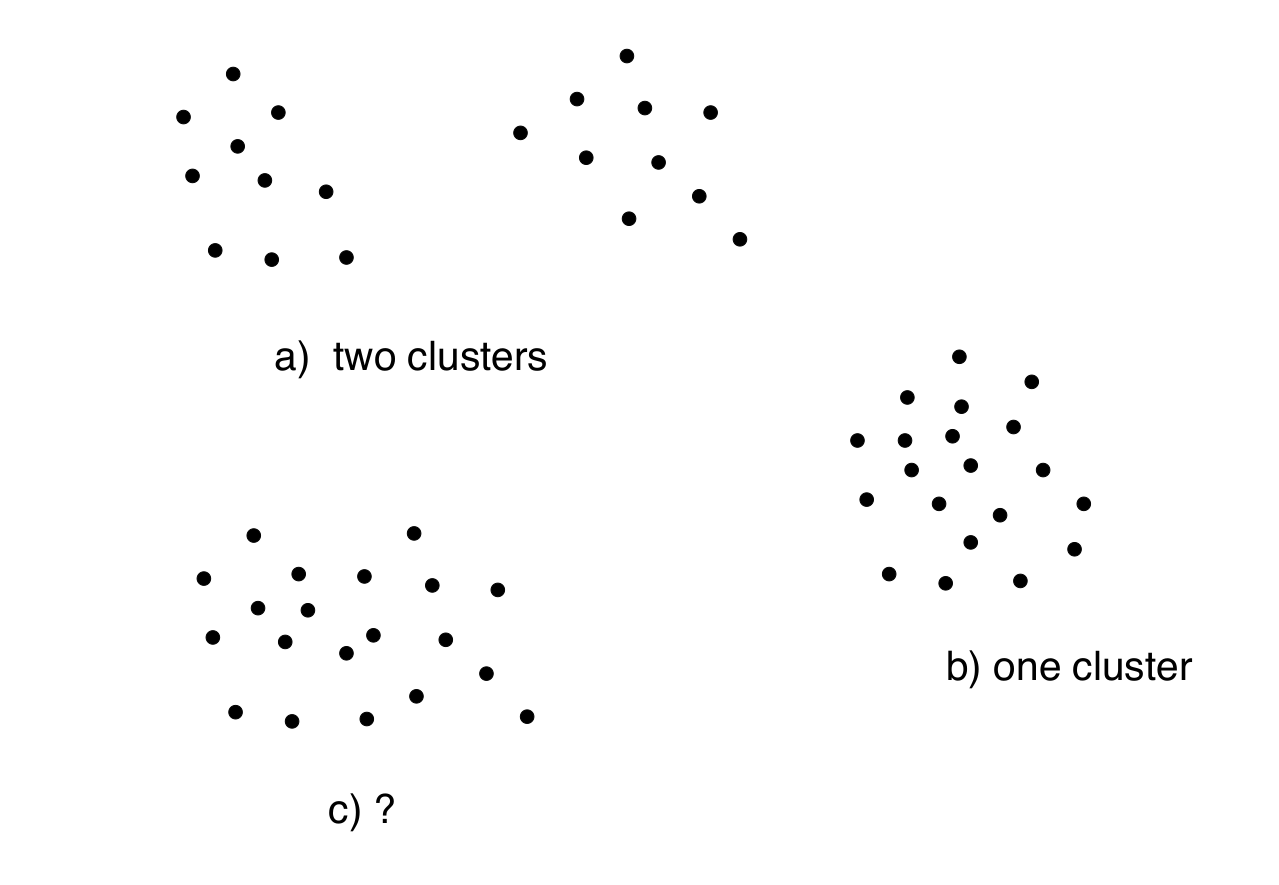
\includegraphics[width=0.85\textwidth]{figs/Unsup_learning.png}
	\caption{vettori di input in uno spazio bidimensionale in tre situazioni differenti. L'immagine è presa da \cite{IntroML}}
	\label{Unsup}
\end{figure}

Quindi un algoritmo di clustering si occupa della suddivisione del set di input $\Sigma$ in un numero N di sottogruppi $\Sigma_1$,...,$\Sigma_n$, detti appunto cluster; si noti che lo stesso numero N non viene stabilito a priori e fornito all'algoritmo, ma viene anch'esso ricavato a partire dai dati. Una volta fatto sarà possibile implementare un classificatore per collegare nuovi vettori di input con i cluster precedentemente individuati.\\
Inoltre, aumentando il livello di complessità, è possibile trovare eventuali gerarchie di partizionamento, ovvero cluster di cluster.

\newpage

\subsection{Metodo di clustering basato sulla distanza euclidea}
\label{metodo distanza euclidea}
Gli algoritmi di apprendimento non supervisionato sfruttano una qualche misura di similarità per separare i pattern (gli input) nei vari cluster. Una possibilità è quella di utilizzare la semplice distanza euclidea per poter separare lo spazio n-dimensionale dei pattern in delle sotto-aree, che sono appunto i cluster. \\
Per fare ciò viene implementato un metodo iterativo, basato sulla definizione di alcuni punti particolari nello spazio dei pattern, detti "cluster seekers" (letteralmente "cercatori di cluster"). \\
Si definiscono M punti nello spazio n-dimensionale $\textbf{C}_\textbf{1},...,\textbf{C}_\textbf{M}$ e l'obiettivo è quello di fare in modo che ogni punto si muova verso il centro di ogni singolo cluster, in modo che ogni cluster abbia al suo centro uno di questi cluster seekers. \\
Come è già stato spiegato precedentemente, l'algoritmo non conosce a prescindere il numero di cluster ma riesce a ricavarlo dai pattern stessi; per questa ragione il numero di cluster seekers M è inizialmente casuale ed esiste un procedura per ottimizzarlo, che verrà illustrata in seguito. \\
I pattern del training data set $\Sigma$ vengono presentati all'algoritmo uno alla volta: per ognuno di essi ($\textbf{x}_\textbf{i}$) si cerca il cluster seekers più vicino ($\textbf{C}_\textbf{k}$) e lo si sposta verso $\textbf{x}_\textbf{i}$ nel seguente modo:
\begin{equation}
\textbf{C}_\textbf{k} + \alpha_k(\textbf{x}_\textbf{i} - \textbf{C}_\textbf{k}) \rightarrow \textbf{C}_\textbf{k}
\end{equation}
dove $\alpha_k$ è un parametro di apprendimento che determina di quanto il cluster seeker k-esimo si muove verso il punto $\textbf{x}_\textbf{i}$. \\
A questo punto è utile fare in modo che più il cluster seeker è soggetto a spostamenti minore diventa l'entità dello spostamento. Per fare ciò si definisce una massa $m_k$ e le si assegna un valore pari al numero di volte in cui $\textbf{C}_\textbf{k}$ è stato soggetto a spostamenti (quindi anche il valore della massa verrà aggiornato di volta in volta); dopodiché si assegna ad $\alpha_k$ il seguente valore
\begin{equation}
	\alpha_k = \frac{1}{1 + m_k}
\end{equation} 
e, dato che ad ogni iterazione che coinvolge $\textbf{C}_\textbf{k}$ il valore di $m_k$ aumenta di una unità, il parametro di apprendimento $\alpha_k$ diminuisce di volta in volta. \\
Il risultato di questo aggiustamento è che il cluster seeker si trova sempre nel punto che rappresenta la media dei punti del cluster. \\
Una volta che sono stati presentati tutti i pattern del training data set all'algoritmo, i vari cluster seeker saranno conversi ai "centri di massa" dei cluster e la classificazione (cioè la delimitazione dei cluster nello spazio n-dimensionale) può essere fatta con una partizione dello spazio di Voronoi, di cui si riporta la seguente definizione:
\begin{quotation} \small
	\textit{In ogni insieme (topologicamente) discreto S di punti in uno spazio euclideo e per quasi ogni punto x, c'è un punto in S che è il più vicino a x. Il "quasi" è una precisazione necessaria dato che alcuni punti x possono essere equidistanti da 2 o più punti di S.
	Se S contiene solo due punti, a e b, allora il luogo geometrico dei punti equidistanti da a e b è un iperpiano, ovvero un sottospazio affine di codimensione 1. Tale iperpiano sarà il confine tra l'insieme di tutti punti più vicini ad a che a b e l'insieme di tutti i punti più vicini a b che ad a. È l'asse del segmento ab.
	In generale, l'insieme dei punti più vicini a un punto c $\in$ S che ad ogni altro punto di S è la parte interna di un politopo (eventualmente privo di bordi) detto dominio di Dirichlet o cella di Voronoi di c. L'insieme di tali politopi è una tassellatura dell'intero spazio e viene detta tassellatura di Voronoi corrispondente all'insieme S. Se la dimensione dello spazio è solo 2, è facile rappresentare graficamente le tassellazioni di Voronoi; è a questo caso che si riferisce solitamente l'accezione diagramma di Voronoi. \\
	(Wikipedia, Diagramma di Voronoi.)} 
\end{quotation}

Un esempio didattico del risultato di questa partizione è riportato in figura ~\ref{Voronoi}.
\begin{figure}[h!]
	\centering
	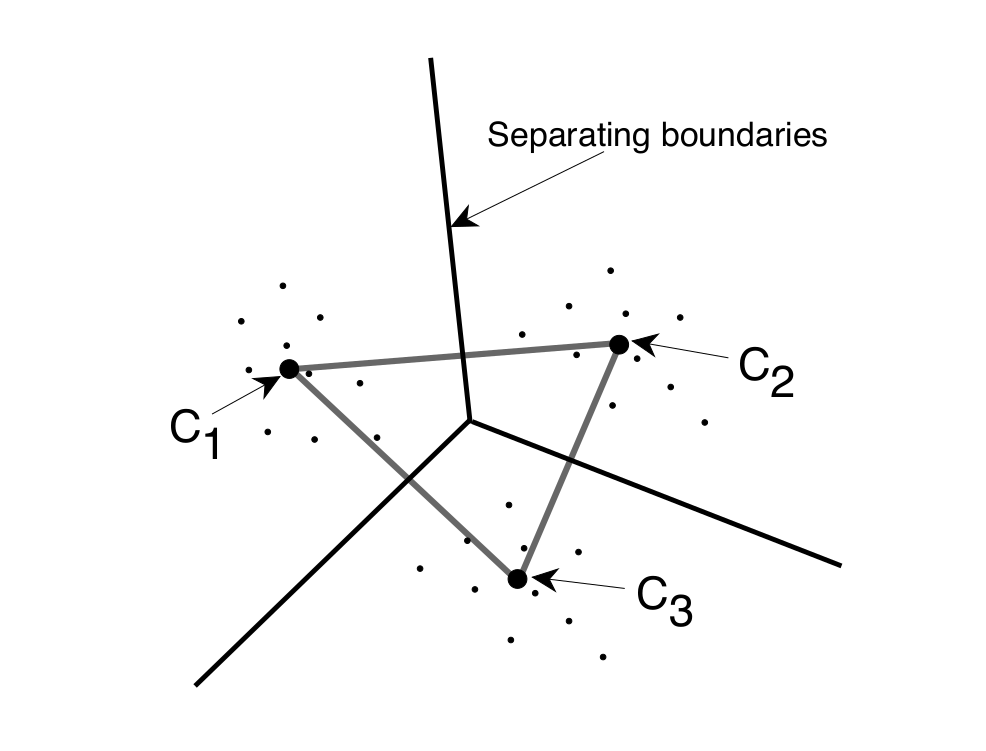
\includegraphics[width=0.70\textwidth]{figs/Voronoi.png}
	\caption{Si riporta un esempio di partizione dello spazio (bi-dimensionale) di Voronoi in tre sotto regioni . L'immagine è presa da \cite{IntroML}}
	\label{Voronoi}
\end{figure}

Si è accennato qualche riga fa che il numero di cluster seeker è inizialmente scelto in maniera casuale, per poi essere ottimizzato; per il processo di ottimizzazione si utilizza la varianza dei pattern $\{\textbf{x}_\textbf{i}\}$ per ogni cluster:
\begin{equation}
	\sigma^2 = \frac{1}{L}\sum_{i=1}^{L} (\textbf{x}_\textbf{i} - \bm{\mu})^2
\end{equation}
dove L è il numero di pattern nel cluster e $\bm{\mu}$ ne è la media:
\begin{equation}
	\bm{\mu} = \frac{1}{L}\sum_{i=1}^{L} \textbf{x}_\textbf{i}
\end{equation}
A questo punto, se la distanza $d_{ij}$ fra due cluster seeker $\textbf{C}_\textbf{i}$ e $\textbf{C}_\textbf{j}$ è minore di un determinato valore $\epsilon$, allora si sostituiscono i due cluster seeker con uno nuovo posto nel loro centro di massa (tenendo conto delle due masse $m_i$ e $m_j$); dall'altro lato, se vi è un cluster per il quale la varianza $\sigma^2$ è più grande di un valore $\delta$, si aggiunge un nuovo cluster seeker vicino a quello già esistente e si eguagliano entrambe le loro masse a zero.\\
Come osservazione finale bisogna dire che nei metodi che si basano sul concetto di distanza è importante ri-scalare i valori delle componenti dei pattern (in linea di principio si possono avere componenti diverse con ordini di grandezza di molto differenti) in modo da evitare che alcune componenti pesino più di altre. \\ 
\newpage